%%%%%%%%%%%%%%%%%%%%%%%%%%%%%%%%
% Title: A Brief introduction to Zotero                                         %                 
% Author: GANG LI                                                                    %
% Institute: Department of Business Administration,                 %
%                Zhongnan University of Economics and Law         %
% Email: gang.li@stu.zuel.edu.cn                                             %
% Github: GangLi-0814                                                             %
%%%%%%%%%%%%%%%%%%%%%%%%%%%%%%%%

\documentclass[UTF8]{beamer}
\usetheme{Pittsburgh} 
\usecolortheme{whale}

\usepackage{graphicx} % insert graphs
\usepackage{hyperref} % hyperlink
\hypersetup{
    colorlinks=true,
    linkcolor=blue,
    filecolor=blue,
    urlcolor=blue,
    citecolor=cyan,
}
\usepackage{multicol} % multicol of Outline
\usepackage{ulem} % delete line

%%%%%%%%%%%%
% Title
%%%%%%%%%%%%
\title{A Brief Introduction to Zotero}
%\subtitle{\textit{A Powerful Tool for Reference Management}}
\author{Gang Li}
\institute{Department of Business Administration\newline  Zhongnan University of Economics and Law}
\date{\today}

\begin{document}

\frame{\titlepage} 

%%%%%%%%%%%%%%%%%
% Self-Introduction
%%%%%%%%%%%%%%%%

%%%%%%%%%%%%
% Outline
%%%%%%%%%%%%
% One Page
\begin{frame}{Outline}
\begin{multicols}{2}
  \tableofcontents
\end{multicols}
\end{frame}

% Beginning of each section
\AtBeginSection[]{
    \frame{\frametitle{Outline}
    \begin{multicols}{2}
    \tableofcontents[sectionstyle=show/shaded,subsectionstyle=show/show/shaded]
      \end{multicols}
        }
}

%%%%%%%%%%
% What's Zotero
%%%%%%%%%%

\section{What's Zotero?}

% Problem
\subsection{Problem}
\begin{frame}{Problem}
\begin{columns}
\begin{column}{.7\linewidth}
\begin{figure}
\centering
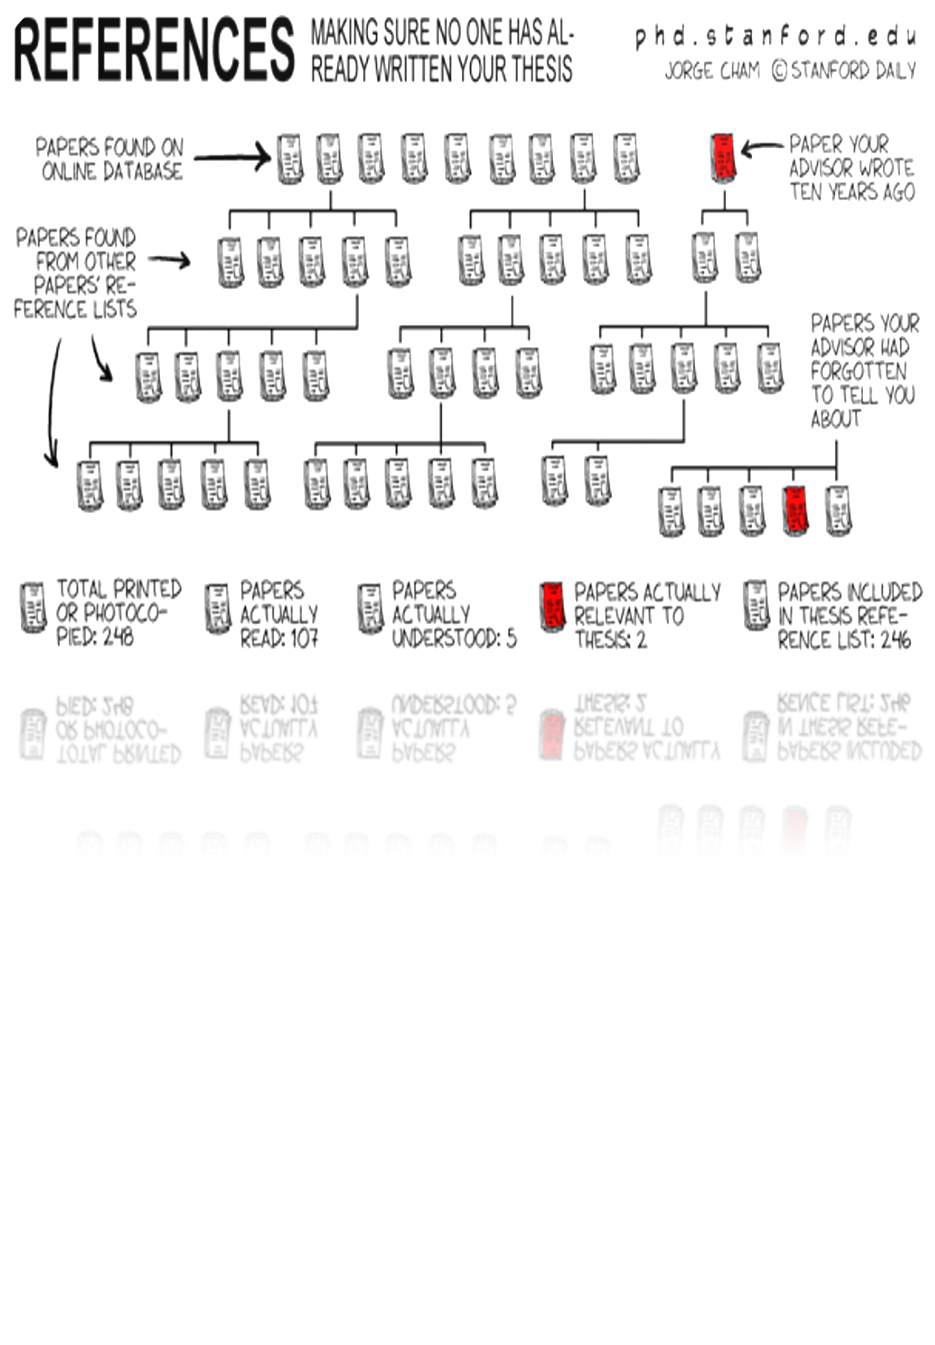
\includegraphics[width=75mm]{figures/information_overskill.png}
\end{figure}
\end{column}
\begin{column}{.3\linewidth}
\textit{How many papers must a man read before we call him a man?}
\end{column}
\end{columns}
\end{frame}

% Options
\subsection{Options}
\begin{frame}{Options}
\begin{figure}
  \centering
  
\includegraphics[width=90mm, height=50mm]{figures/different_tools.jpg}
 \end{figure}
\begin{itemize}
\item Question: Which one do you perfer?
\item My Answer: \textit{Zotero.}
\end{itemize}
\end{frame}

% My Answer
\begin{frame}{Introduction}
\begin{columns}
\begin{column}{.3\linewidth}
\begin{figure}
\centering

\includegraphics[width=30mm]{figures/Zotero_icon.png}
\end{figure}
\end{column}
\begin{column}{.7\linewidth}
\begin{itemize}
\item Zotero is, at the most basic level, a reference manager.
\item It is designed to \textbf{\textcolor{blue}{store, manage and cite}} bibliographic references, such as books and articles.
\item More broadly, Zotero is a powerful tool for collecting and organizing research information and sources.
\end{itemize}
\end{column}
\end{columns}
\end{frame}

%%%%%%%%%%
% Why Zotero
%%%%%%%%%%

\section{Why Zotero?}

%Comparison
\subsection{Comparison}
\begin{frame}{Comparison}
%\begin{itemize}
%\item Wikipedia: \href{https://en.wikipedia.org/wiki/Comparison_of_reference_management_software}{\color{blue}{Comparison of reference management software}}
%\item UChicago Library Guides: \href{https://guides.lib.uchicago.edu/c.php?g=297307&p=1984557}{\color{blue}{How to Choose a Citation Manager}}
%
%\end{itemize}
\begin{figure}
\centering
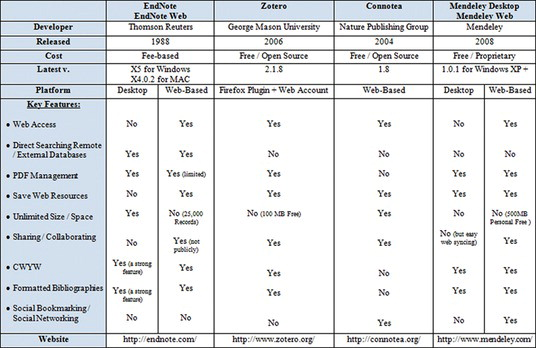
\includegraphics[width=100mm]{figures/comparison.jpeg}
\end{figure}
\tiny
Source: ZHANG Y. Comparison of Select Reference Management Tools[J]. Medical Reference Services Quarterly, Routledge, 2012, 31(1): 45–60.  
\href{https://www.tandfonline.com/doi/full/10.1080/02763869.2012.641841?scroll=top&needAccess=true}{\color{blue}{[click here]}}
\end{frame}

% Features
\subsection{Features}
\begin{frame}{Features}
\begin{enumerate}
\item Free and Open Source
\item Tags
\item Groups
\item Saved Searches
\item LookUp Engines
\item \textit{RSS} Feeds
\item Zotero + Sci-hub
\item Zotero + Web of Science
%\item PDF Preview
%\item Zotero + Connected Papers
%\item Different Types of Resources
%\begin{itemize}
%\item Journal articles
%\item Book chapters
%\item Newspaper articles
%\item Webpages
%\end{itemize}
\end{enumerate}
\end{frame}


%%%%%%%%%%
% Install
%%%%%%%%%%
\section{How to Install?}

% Set up
\subsection{Set up}
\begin{frame}{Set up}
\begin{enumerate}
\item Download
  \begin{itemize}
  \item Open the \href{https://www.zotero.org/download/}{\textit{\color{blue}\underline{Download Page}}}
  \item Zotero
  \item Browser Extension
  \end{itemize}
\item Install
    \begin{itemize}
    \item Zotero: click \textbf{next} until the installation is complete
    \item Extension: If failed, try offline installation
    \end{itemize}
\item Read the \href{https://www.zotero.org/support/quick_start_guide}{\textit{\color{blue}\underline{Quick Start Guide} } }
%\item Open Zotero and select a referencing style
%\item Keep Zotero open in the background while you browse for resources online
\end{enumerate}
\end{frame}

%% Install
%\subsection{Install}
%\begin{frame}{Install}
%\begin{itemize}
%\item item1
%\item item2
%\end{itemize}
%\end{frame}

% Configuration
\subsection{Configuration}
\begin{frame}{Configuration}
\begin{enumerate}
\item Settings
  \begin{itemize}
  \item Switch language
  \item Install Microsoft Word Add-in
  \item Classic View
  \end{itemize}
  
\item Useful Extensions

  \begin{itemize}
    % ZotFile
  \item  \href{http://zotfile.com/}{\color{blue}ZotFile}
    \begin{itemize}
    \item Advanced PDF management for Zotero
    \end{itemize}
    % jasminum
   \item \href{https://github.com/l0o0/jasminum}{\color{blue}{Jasminum}}
   \begin{itemize}
   \item A Zotero add-on to retrive CNKI meta data
   \end{itemize}
   % ZoteroQuickLook 
  \item \href{https://github.com/mronkko/ZoteroQuickLook/releases}{\color{blue}ZoteroQuickLook}
  % Zutilo
  \item \href{https://github.com/wshanks/Zutilo}{\color{blue}{Zutilo}}
  \begin{itemize}
  \item Add extra menu items and keyboard shortcuts
  \end{itemize}
  % markdown-here
  \item \href{https://github.com/fei0810/markdownhere4zotero}{\color{blue}markdowm-here}
 % scite
 \item \href{https://github.com/scitedotai/scite-zotero-plugin}{\color{blue}scite}
  \end{itemize}
\end{enumerate}
\end{frame}

%%%%%%%%%%
% Usage
%%%%%%%%%%

\section{How to Use?}

% Basic Usage
\subsection{Basic Usage}

%% Layout
\begin{frame}{Layout}
\begin{itemize}
\item Layout
  \begin{itemize}
  \item Left-hand column: arrange collections into folders. 
  \item Middle column: shows the content of these folders.
  \item Right-hand column: browse, and edit the detail of the individual item.
  \end{itemize}
\end{itemize}
\end{frame}

\begin{frame}{Importing Resources}
\begin{itemize}
\item Creating folders and searching Zotero
 \item Adding resources to your collection
   \begin{itemize}
   \item Adding automatically through web pages 
   \item Adding by identifier
   \item Adding items manually
   \item \href{https://www.zotero.org/support/moving_to_zotero}{\textit{\color{blue}{Importing from other reference managers}}}
   \item \href{https://www.zotero.org/blog/scan-books-into-zotero-from-your-iphone-or-ipad/}{\textit{\color{blue}{Scan Books into Zotero from Your iPhone or iPad}}} 
   \item Moving from other reference managers (e.g. \href{https://libguides.nus.edu.sg/c.php?g=145733&p=1433183}{\color{blue}{Endnote}})
  \end{itemize}
\item Duplicate items
\end{itemize}
\end{frame}

%% Citation
\begin{frame}{Citation}
\begin{itemize}
\item Citation Style
    \begin{itemize}
    \item How to define citation style you want to use
    \item How to find and add citation style
    \item How to modify citation style \href{https://editor.citationstyles.org/visualEditor/}{\textit{\color{blue}{[Visual CSL Editor]}}}
    \item \textbf{\color{red}{Trouble: GB/T 7714-2015}} 
   	\begin{itemize}
	\item What's GB/T 7714-2015? \href{http://manu49.magtech.com.cn/journalx_gdgyzrb/UserFiles/File/GBT7714-2015.pdf}{\textit{\color{blue}{[GBT 7714-2015.pdf]}}}
	\item Where is the trouble with Zotero?
	\end{itemize}
  \end{itemize}
\item Multiple Sources
\item Creating a Bibliography
\end{itemize}
\end{frame}

% Advanced Usage
\subsection{Advanced Usage}
\begin{frame}{Advanced Usage}
\begin{itemize}
\item Tags
\item Groups
\item Saved Searches
\item LookUp Engines
\item \textit{RSS} Feeds
\item Zotero + Sci-hub
\item Zotero + Web of Science
\item PDF Preview
%\item Zotero + Connected Papers
\end{itemize}
\end{frame}

%%%%%%%%%
% Information
%%%%%%%%%
%\begin{frame}
% \begin{center}
%{\huge \emph{\textcolor{blue}{Thank  ~you!}}}\\
%\vspace{5mm}\large
%\begin{tabular}{ll}
%{\sc Author}:  & GANG Li\\
%{\sc Address}: &Department of Business Administration\\
%               & Zhongnan University of Economics and Law\\
%               & Wuhan, 430073, China\\
%  {\sc Email}: & \href{mailto:gang.li@stu.zuel.edu.cn}{\color{blue}gang.li@stu.zuel.edu.cn}\\
%\end{tabular}
%\end{center}
%\end{frame}

\begin{frame}{Contact}
\begin{columns}
\begin{column}{.4\linewidth}
\begin{figure}

\includegraphics[width=40mm]{figures/Wechat_QR.jpeg}
\end{figure}
\end{column}
\begin{column}{.6\linewidth}
{\huge \emph{\textcolor{blue}{Thank  ~you!}}}\\
\vspace{5mm}\large
\begin{tabular}{ll}
{\sc Author}:  & GANG Li\\
{\sc Github}: & \href{https://github.com/GangLi-0814}{\color{blue}{GangLi-0814}}\\
{\sc Blog}: & \href{http://lgspace.top}{\color{blue}http://lgspace.top}\\
{\sc Email}: & \href{mailto:gang.li@stu.zuel.edu.cn}{\color{blue}gang.li@stu.zuel.edu.cn}\\
\end{tabular}
\end{column}
\end{columns}
\end{frame}


\end{document}


